\documentclass[letterpaper,10pt,serif,draftclsnofoot,onecolumn,compsoc,titlepage]{IEEEtran}

\usepackage{graphicx}                                        
\usepackage{amssymb}                                         
\usepackage{amsmath}                                         
\usepackage{amsthm}                                          
\usepackage{cite}
\usepackage{alltt}                                           
\usepackage{float}
\usepackage{color}
\usepackage{url}

\usepackage{balance}
\usepackage[TABBOTCAP, tight]{subfigure}
\usepackage{enumitem}

\usepackage{geometry}
\geometry{margin=.75in}
\usepackage{hyperref}
%\usetikzlibrary{shapes, positioning, calc}
\usepackage{caption}
\usepackage{listings}
%\usepackage[utf8]{inputenc}
%pull in the necessary preamble matter for pygments output

%% The following metadata will show up in the PDF properties
% \hypersetup{
%   colorlinks = false,
%   urlcolor = black,
%   pdfauthor = {\name},
%   pdfkeywords = {cs311 ``operating systems'' files filesystem I/O},
%   pdftitle = {CS 311 Project 1: UNIX File I/O},
%   pdfsubject = {CS 311 Project 1},
%   pdfpagemode = UseNone
% }

\parindent = 0.0 in
\parskip = 0.1 in
\title{Spring Mid Term Progress Report}
\author{Shannon Ernst, Kyle Nichols, Javier Franco\\ Group 48 \\ 15 May 2017 \\ CS 463 Spring 2017}
\begin{document}
\maketitle
\begin{abstract}

\end{abstract}
\newpage
\tableofcontents
\newpage
\section{Purposes and Goals}
The STEM Academy program in Corvallis, Oregon, seeks to provide education in science, technology, engineering and math to the K-12 community through various programs, campus, and clubs.
They are self funded, relying on grants, donations and other sources, many of which require results-based data on the success of STEM Academy programs.
This data is collected from surveys that participants take while they are enrolled in one of STEM Academy's camps and other programs.
Currently, these surveys are administered on paper and the responses are tabulated by hand by volunteers.
This has not been an effective way of collecting current data to help secure funding and many of the surveys go untabulated.
The STEM Academy does have the ability to register participants online through Ideal Logic, but this is this does not help them with tabulating survey data.
They need a system which will allow them to electronically create surveys, a database to house all of the data from those surveys, and a report generation system so they can view the most current data in a timely and meaningful way.

A website which will allow the STEM Academy to create and distribute surveys, as well as view helpful data results, is the best solution.
The website should allow them to create questions that can be included across multiple surveys.
The questions should be able to be templated so that only one part of the question need change according to the topic of the survey.
Surveys should be able to be distributed via a web link or printed.
After a survey is taken, the data should be stored in a database according to the type of program.
This data should be queriable based on custom queries.
The user should be able to make a query based on the question and collected demographics as well as filter by program.
This service should be user friendly; the user should not need to know any SQL or other querying language in order to get data from the database.
After a query, the data should be able to be saved and added to a printable report so that it can actually be used in grant proposals and marketing material.
This website will be an all in one package for collecting and reporting on data in a timely fashion which is what the STEM Academy truly needs.
By the Engineering Expo, we will be able to present this website and show the full path of data collection, from creating the survey to querying to report generation.

\section{Current Status}
The current status of our project is that we finished our web application and it functions properly. We are waiting on getting more feedback from our clients to see if they found any bugs that we need to fix and also any minor changes that they would like us to make. We finished our poster for expo on time and we will be receiving it during the week of expo. We are ready to present at expo and we are going to be running a video in the background that demonstrates the functionality of our web application. 

\section{Left To Do}
The things that remain to do are to meet up with our clients to transfer the project, documentation, and to give them training on how to use the web application. We have already sent them an email and we are currently waiting on a response on what day and time in early June works for them. While we wait to meet up with our clients we will be updating all of our documentation, so that it reflects the changes that we made. We still need to record a video of how our web application works to run in the background in one of our computer's for expo and we are planning on doing this early this up coming week. This will be an easy task to accomplish and it should not take a long time to do.

\section{Retrospective}
\begin{center}
    \begin{tabular}{ | p{5cm} | p{5cm} | p{5cm} |}
    \hline
     Positive & Delta & Action \\ \hline
     We all attended the TA meetings and we were also on time. & When our client sends us a message we need to respond more quickly. & If the person who is the main point of contact is not able to respond to the client the other group members should respond in order to provide them with a timely response. \\ \hline

     

     
    \end{tabular}
\end{center}

\section{Term Break Down}
\subsection{Week 1}
This week we met with our client. We implemented the survey taking portion which included: 
populating camp drop down by date on student log in,
populating student drop down by selected camp on student log in,
generate survey for student to take based on provided info,
store the responses of the taken survey. These required us to create new json objects. 
The down side to this week is we are slightly late on this as we were hoping to have it to our client on Monday.
 We are still working with Central Services who appear to be ignoring our attempts at communication.
 Next week our client will be able to play with the product and see what they like and don't like.
 This week, on Monday, Kyle helped Shannon with finalizing the survey taking component of our project.
Kyle also made several changes to the database structure. The Camp table now contains an enrollment array
 of Responder IDs for students enrolled in the camp. This change is also reflected by updating the
 addCamp.php page to do this when uploading enrollment CSV files. The Responder table was updated
 with new demographic information: ethnicity, race, free or reduced lunch status, and the highest
 level of education one of their guardians obtained. This demographic information comes from STEM Academy's
 demographic surveys on IdealLogic and is important to how they collect data.
Next week we will finish development and begin polishing our code. This will likely include,
 on my part, adding some error handling to database interaction code (for example, handling adding 
 duplicates to the database).
This week Javier fixed a bug that was in the create a new report web page that created a new row in 
the Report table each time a new report was saved or changes were saved. Javier also made some changes
 to the delete admin web page to prevent the accounts of our clients from being deleted by other admin
 users including themselves. This week Javier has also been working on the implementation of the returning
 a query result, but this is a difficult and tedious task. Right now Javier is almost done with returning
 a result for using regular query templates. After getting this done Javier will have to deal with the
 change in response query template and also filtering the query results based on the demographic
 information that was selected. Furthermore, Javier has to fix a bug in his query template drop downs
 and also create nested drop downs for matrix questions. All of this will take time to implement, so Javier
 is hoping that nobody rushes or pressures me to finish all of this because Javier still have to deal with
 three hw assignments for his other classes.
\subsection{Week 2}
This week Shannon got Central Service to finally give us our website. We have everything
 allocated so we can start moving things over. We have been struggling to complete development.
 Javier has been having a hard time understanding the querying process so Shannon sat down with
 him to help him refactor his code. This took a long time as he struggled with understanding the
 underlying logic of reusing data collected from the database and using json objects. Meanwhile, Kyle
 was going through removing bugs from our code and managed to break a section of my code. It is unclear
 what he did and we attempted to roll back to a previous commit but it doesn't seem to have worked.
 The drop down menus are still broken. This weekend Shannon will be hauling the project into a complete state,
 Shannon will be fixing whatever issue Kyle caused and Shannon will be finishing Javier's code.
 The only blocker is Kyle deleted data from our database which is critical to testing so Shannon will
 have to add more data to the database. Shannon will be finishing our poster draft over the weekend.
 We still haven't contacted our client through this entire debacle and they have not contacted us.
 Things will be tight this next week. Edit: Kyle's issue was a permissions one. Nothing is broken
 which is a relief.
 This week Kyle met with the team to work on some polishing while Shannon and Javier worked on finishing
 the report generation. Kyle developed a verification on the randomly generated IDs to make sure that the
 ID being inserted doesn't exist already in the database. If this isn't done, you'd (rarely, but increasingly
 with the size of the database) get an error from inserting a pre-existing ID.
However, in adding this and some more polishing work, Kyle noticed a bug where in the drop-down menu for
 frequently-used questions where matrix questions were listed as blank. In trying to fix this bug Thursday night,
 the drop-down menus for the survey creation page suddenly stopped working, which prevented any functionality
 of adding questions. Ultimately, the next morning we realized this was a permissions issue (we don't know how 
 this had changed so suddenly). It is currently resolved, but since I reverted all of my changes Thursday night
 to try and fix this sudden bug, my progress on polishing and the ID verification code was removed.
This weekend and early next week Kyle should be able to add that code back since luckily it was pretty short.
 Kyle will also next week start preparing the database on Central Web Services since the domain and MySQL
 database have now been provided.
 This week Javier worked with Shannon on refactoring my code because it was not readable enough what Javier was
 doing which made it difficult for her to understand with what was going on. While refactoring my code we
 discussed our approaches for doing the querying which were different and she helped clear things up.
 She also showed me the proper way to make a JSON object into a string how to decode the string form
 properly in order to get the JSON object's values. This helped with removing unnecessary variables that Javier
 was creating. She plans on finishing my code up over the weekend, so that we can send a link to our client
 as soon as possible to have them test our web application and also to transfer over central services. The reason
 why my code was not readable is due to not have any previous experience with JSON objects and DOM manipulation
 because Javier learned all of this on the fly last term. Another thing that Javier noticed was that Shannon's 
 experience with creating web application's allows her to come up with quick solutions for DOM manipulation that
 seem complicated for me to implement, but after she explains solution its easy to implement.
\subsection{Week 3}
Last week Shannon was working with Javier to get the report generation working. The issue is that,
 though he is a hard worker, he gets too caught in the syntax and does not know what problem he is
 actually solving. His code is also completely unmanageable in style with too many comments and
 unneeded variables. With my limited time, Shannon could not sit down and help him as much this week
 so she asked him to push the code to her so she could just finish it. He did so but then continued to
 work on it leaving her with the impression that he was going to finish it. This was not the case and 
 when they discussed after lecture what was left to be done (all of which the code had already been 
 written for in survey generation, it just needed to be adapted for reports) he said he could not 
 accomplish it without more research and sitting down with me. This caused Shannon some frustration as
 she could not understand why he could not find the appropriate code in her work and adapt it. She then
 told him to give her what he had done and she would finish it. On attempting to do so she made the
 decision to give the client what they had right now as all of Javier's code needs to be heavily refactored
 and she did not want to add code yet. Unfortunately she still has not had time to work on it as she was working
 an event all weekend. The client is aware of where we stand and she will be pulling late nights this week
 to make the May 1 code freeze.
 This week Kyle did some debugging and polishing of code with the team. On my work, there weren't really
 any problems encountered, but as a whole, our team is running into unforeseen problems as a whole in 
 finalizing report generation that has delayed us behind where we anticipated being.
Next week Kyle will likely spend some more time polishing and testing the product.
This week Javier spent numerous hours working on the report generation page Javier was able to fix
 the drop down bug that prevented a user from clicking on a drop down option thanks to Shannon's advice.
 Javier was able to implement the querying for returning a result for a matrix, text entry, and multiple
 choice question. This took a significant amount of time due to changing JSON object that contained the
 PHP query results and also with verifying that they were the correct results. The pseudo code that Shannon
 provided Javier with helped Javier with setting up the text entry and multiple choice results. After Javier got the
 results for these two questions types I then had to figure out how to return the results for a matrix question.
 The matrix question results took the longest due to the format that Javier wanted to display which was the primary
 question along with the sub questions with their corresponding results. In addition, Javier had to create a function
 to return a percentage or a count based on the user's selection. Another thing that Javier had to change was the query
 drop downs for the matrix and text questions, so that it only displayed the question. In order to send the client
 the link to test our webpages Shannon took over where Javier left at and did an excellent jo. Javier is very thankful
 that she did this and also for his teams patience. Over the weekend Javier will check if anything still remains
 for the report generation page, so that it can be completed before we demo our web app to our TA.
\subsection{Week 4}
This week has been concerned with administration issues. We met with the TA to get feedback on our project.
 Javier and Shannon met briefly to confirm progress on the report generation. It seems like everything is
 wrapping up nicely. The poster was completed and Kyle received a signature for it. Shannon collected the photo
 release forms and will be turning them into Covell as well as turning in the poster to the printer.
 Even though code freeze is on Monday, we will be transferring the code to Central Services through out
 May and essentially using May to make sure our clients are set up for the summer. We are set for Expo.
 This week Kyle worked primarily on the editing and revising the poster to get it into a working form for
 our final submission. Kyle also got the signatures from my client and teammates.
 This week Javier finished the remaining parts of the report generation page from last week that Javier
 still needed to do which included being a able to save a report, edit a report, delete a table query,
 and print a report. The reason why there was this many things left was due to changes Javier made to the
 page for returning query results for text and matrix questions. Shannon was not able to refactor my code
 to finish the remaining parts due to how poorly I wrote my code which included adding to many unnecessary
 comments. The style sheet that she added to the report generation helped with making the page look
 aesthetically pleasing and also with printing the report which reduced the amount of work Javier had to do.
 The only things that remain is to test the web pages to see if their are any minor bugs before the code
 freeze and Javier also need to check the other code files that Javier wrote, so that Javier can remove
 any unnecessary comments, echo statements, and inner HTML statements that Javier used for testing. Javier
 think our group is in a great position and we are on track with completing our promised product for our clients.
\subsection{Week 5}
This week not much occurred. The code freeze was met perfectly fine. We got some feedback from our
 client on a minor bug that did not effect code freeze. We will be working between now and the end
 of term to move everything over to Central Services. The poster for Expo was submitted on time.
 Everything is coming together nicely.
 Kyle met with his team on Wednesday to evaluate where we are at. As far as my work toward Capstone 
 this week, Kyle was only able to work on the WIRED interview.
 This week not a lot happened. We had a meeting to discuss where we are in our project and decided
 that we are meeting the up coming week to transfer the web pages to central services. Javier is
 hoping that we get more feedback from the clients, so that we make any changes to the webpages to
 meet their needs and also to fix any bugs that they find.
\subsection{Week 6}
This week Shannon contacted our client to set up a meeting to transfer the project. She has yet to hear back from our client. She also set up the mid term progress report document and the slides for the presentation. She mentioned that we still need to create a video demo to run our project for expo and that we will be also transferring things to Central Services web space. This week Kyle worked on generating the new tables for the Central Web Services hosted database to match our current tables. They are currently still empty. He also worked with Javier on adding some functionality for editing camps that our clients need.

\newpage
\section{Images of Project}

\begin{figure}[!htbp]
\centering

\includegraphics[scale=.9]{ProjectImages/IndexPage.png}
\caption{Starting Page for a Student and Admin}
\label{fig:code2}
\end{figure}

\begin{figure}[!htbp]
\centering
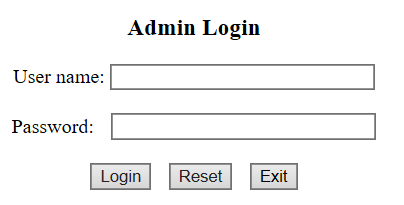
\includegraphics[scale=.9]{ProjectImages/AdminLogin.png}
\caption{Admin Login Page}
\label{fig:code2}
\end{figure}

\begin{figure}[!htbp]
\centering
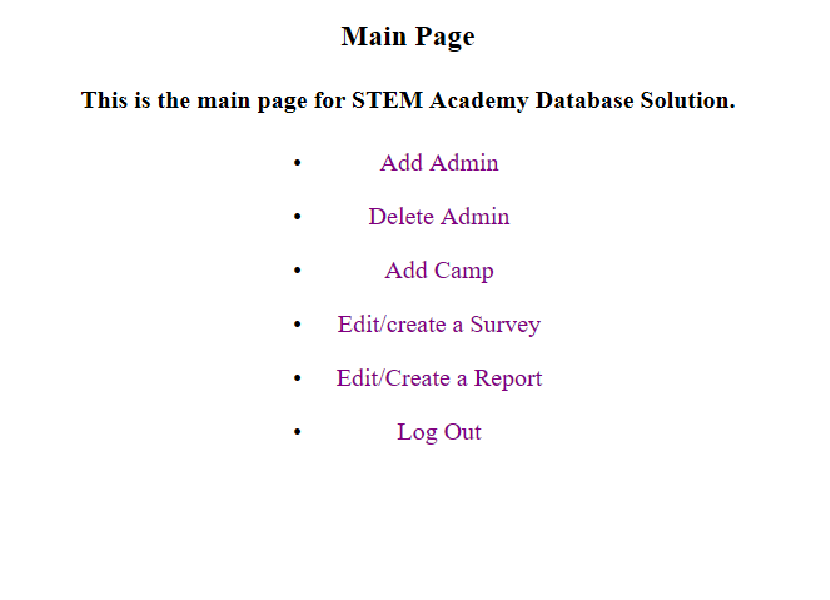
\includegraphics[scale=.2, width=100mm]{ProjectImages/Dashboard.png}
\caption{Dashboard Options Page for Admin Users}
\label{fig:code2}
\end{figure}

\begin{figure}[!htbp]
\centering
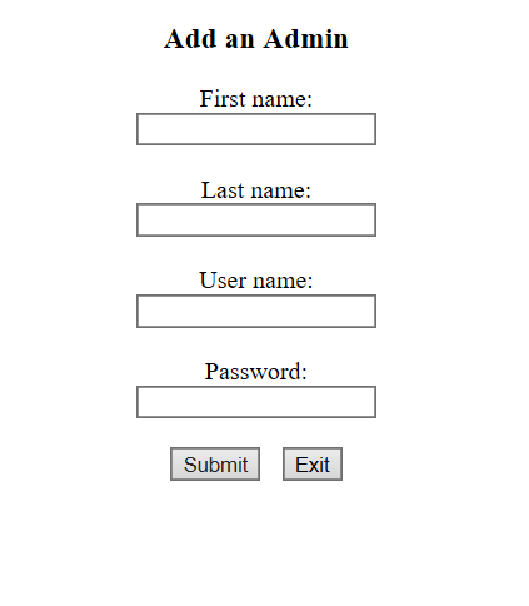
\includegraphics[scale=.9]{ProjectImages/AddAdmin.png}
\caption{Add a New Admin Page}
\label{fig:code2}
\end{figure}

\begin{figure}[!htbp]
\centering
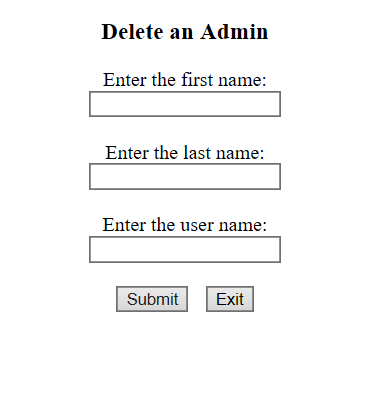
\includegraphics[scale=.9]{ProjectImages/DeleteAdmin.png}
\caption{Delete an Admin Page}
\label{fig:code2}
\end{figure}

\begin{figure}[!htbp]
\centering
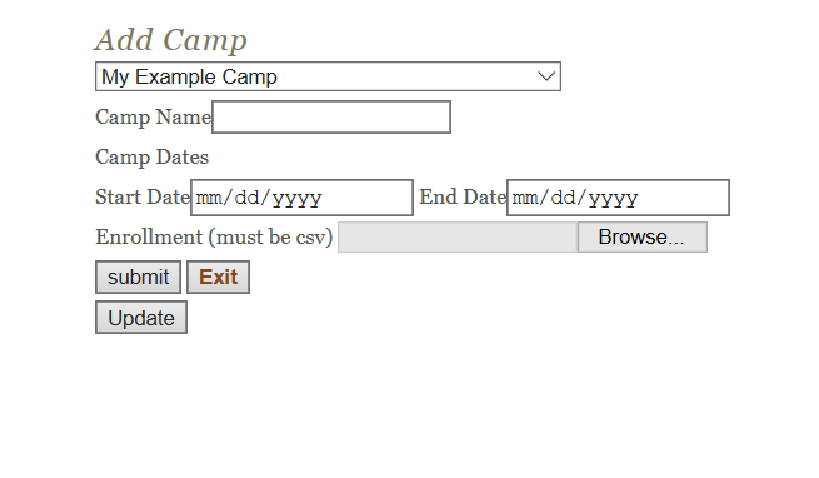
\includegraphics[scale=.2, width=100mm]{ProjectImages/AddCamp.png}
\caption{Add a New Camp Enrollemnt Page}
\label{fig:code2}
\end{figure}  

\begin{figure}[!htbp]
\centering
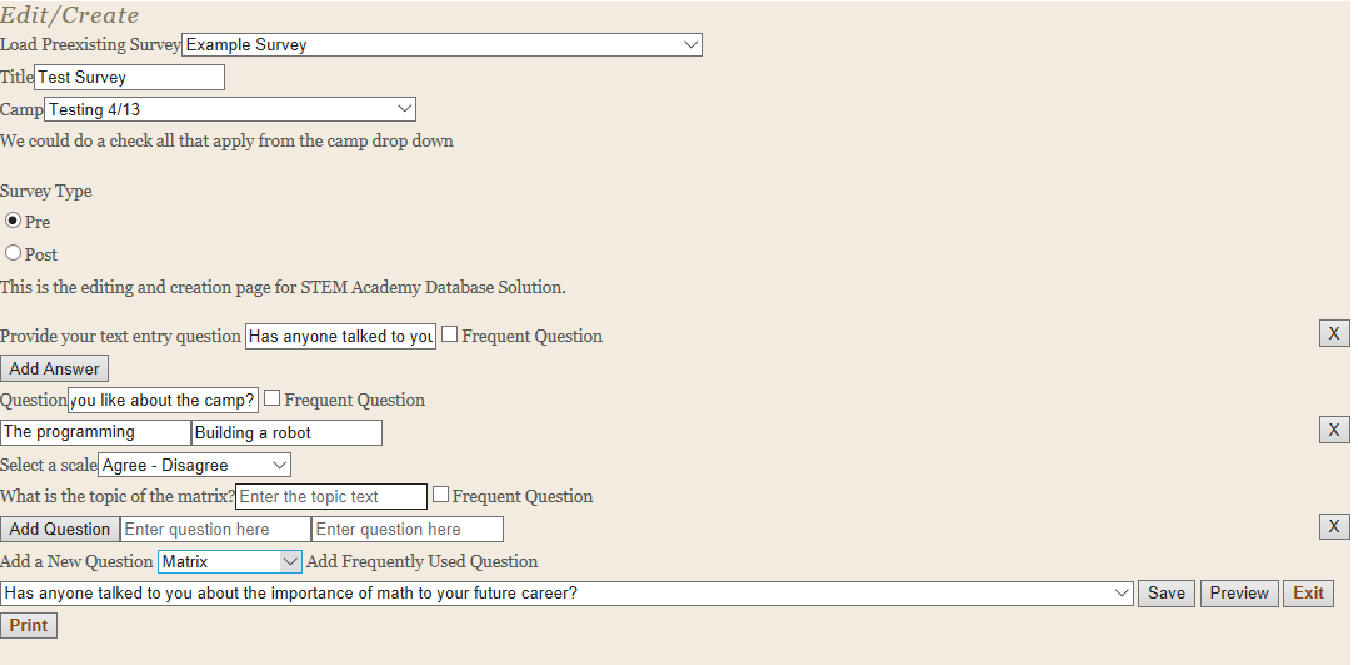
\includegraphics[scale=.8]{ProjectImages/SurveyGeneration.png}
\caption{Generating a New Survey Page}
\label{fig:code2}
\end{figure}  

\begin{figure}[!htbp]
\centering
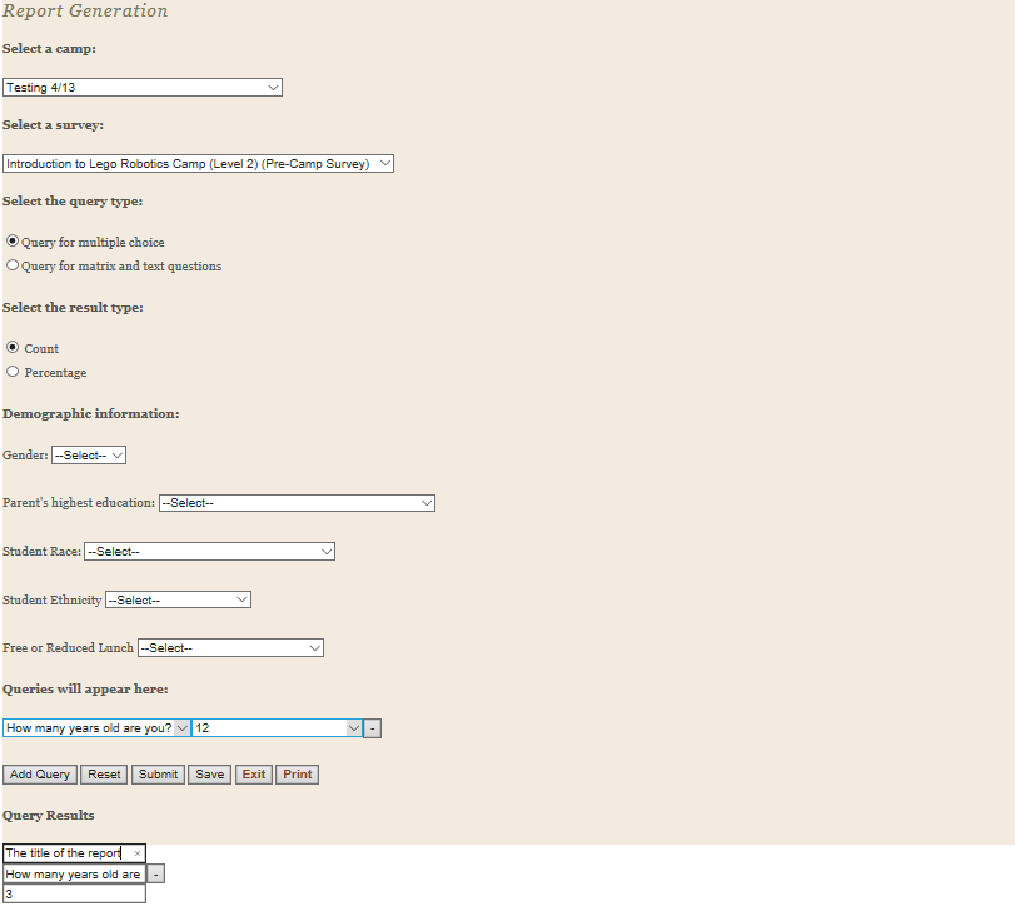
\includegraphics[scale=.9]{ProjectImages/ReportGeneration.png}
\caption{Generating a New Report Page}
\label{fig:code2}
\end{figure}  

\begin{figure}[!htbp]
\centering
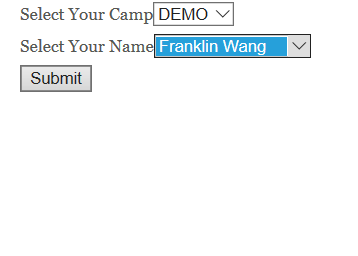
\includegraphics[scale=.9]{ProjectImages/StudentLogin.png}
\caption{Student Selection Page for Taking a Survey}
\label{fig:code2}
\end{figure}  

\begin{figure}[!htbp]
\centering
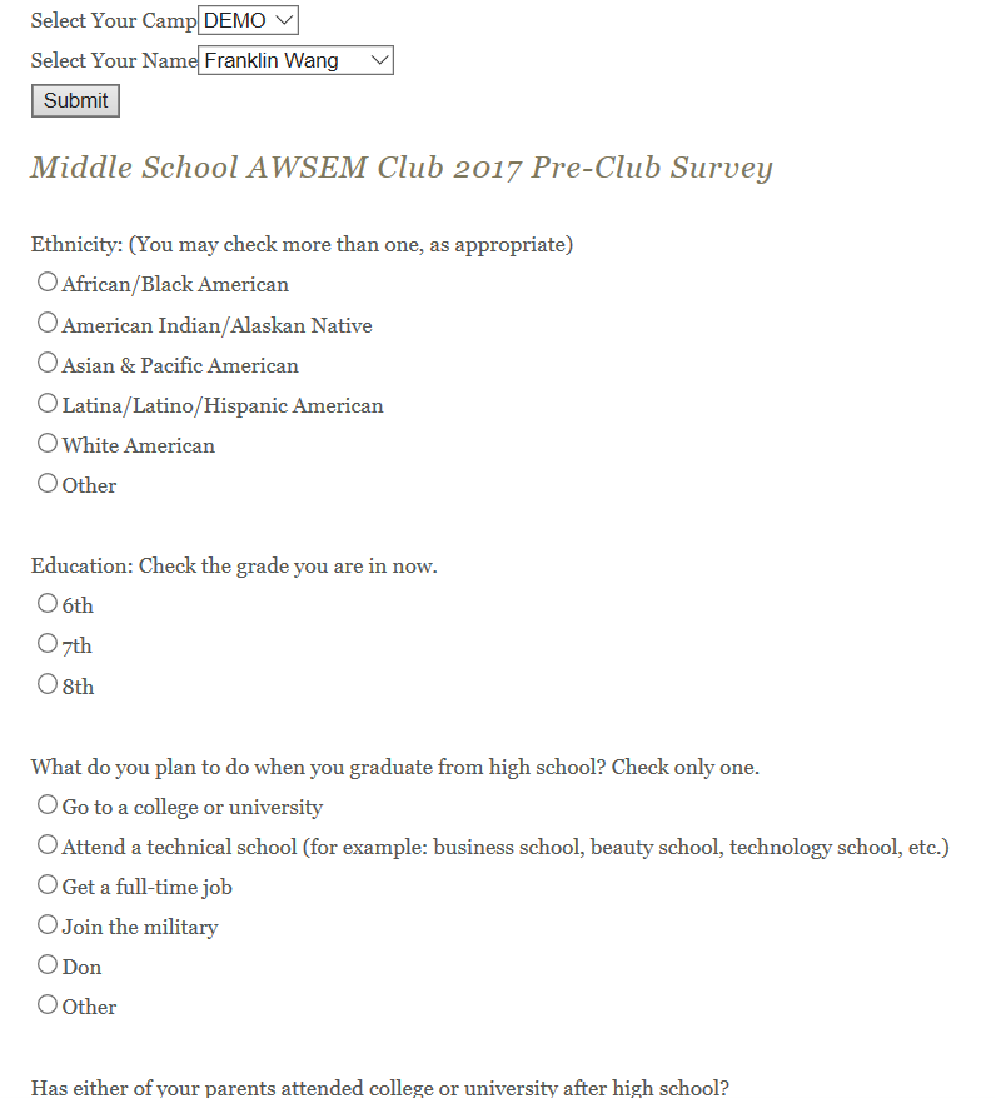
\includegraphics[scale=.2, width=100mm]{ProjectImages/StudentTakingSurvey.png}
\caption{Student Taking a Survey Page}
\label{fig:code2}
\end{figure}  


%\bibliographystyle{ieeetr}
%\bibliography{writing1}
\end{document}
